\documentclass{article}
\usepackage{graphicx} % Required for inserting images
\usepackage{tikz}
\usepackage{svg}

\title{Problem Set 1}
\author{Aleksandr Efremov}
\date{July 2023}

\begin{document}

\maketitle

\section{Part II}
\subsection{Problem 1}
\[
\frac{x-1}{x+1} = \frac{(x-1)(x-1)}{(x+1)(x-1)} = 
\frac{(x-1)^2}{x^2-1} = \frac{x^2-2x+1}{x^2-1} =
\frac{x^2+1}{x^2-1}+\frac{-2x}{x^2-1}
\]

where \(\frac{x^2+1}{x^2-1}\) is even and \(\frac{-2x}{x^2-1}\) is odd

\subsection{Problem 2}


\tikzset{every picture/.style={line width=0.75pt}} %set default line width to 0.75pt        

\begin{tikzpicture}[x=0.75pt,y=0.75pt,yscale=-1,xscale=1]
%uncomment if require: \path (0,300); %set diagram left start at 0, and has height of 300

%Straight Lines [id:da5723816642656105] 
\draw    (161,231) -- (529,230.5) ;
%Straight Lines [id:da44408248612212287] 
\draw  [dash pattern={on 0.84pt off 2.51pt}]  (262,124.5) -- (262,232) ;
%Shape: Circle [id:dp4893111353532078] 
\draw   (237,99.5) .. controls (237,85.69) and (248.19,74.5) .. (262,74.5) .. controls (275.81,74.5) and (287,85.69) .. (287,99.5) .. controls (287,113.31) and (275.81,124.5) .. (262,124.5) .. controls (248.19,124.5) and (237,113.31) .. (237,99.5) -- cycle ;
%Straight Lines [id:da6905923948272086] 
\draw    (262,124.5) -- (423,231.5) ;

% Text Node
\draw (248,240) node [anchor=north west][inner sep=0.75pt]   [align=left] {$\displaystyle x_{0}$};
% Text Node
\draw (246,45) node [anchor=north west][inner sep=0.75pt]   [align=left] {Satellite};
% Text Node
\draw (418,237) node [anchor=north west][inner sep=0.75pt]   [align=left] {$\displaystyle x$};
% Text Node
\draw (342,149) node [anchor=north west][inner sep=0.75pt]   [align=left] {$\displaystyle h$};
% Text Node
\draw (321,240) node [anchor=north west][inner sep=0.75pt]   [align=left] {$\displaystyle L$};
% Text Node
\draw (201,169) node [anchor=north west][inner sep=0.75pt]   [align=left] {$\displaystyle 20000$};
\end{tikzpicture}

\[L = \sqrt{h^2-20000^2}\]

\begin{itemize}
    \item[a)] 
\[h_0 = 25000, L_0 = \sqrt{25000^2-20000^2} = 15000\]
\[\Delta h = 1, h = 25001, L = \sqrt{25001^2-20000^2} \approx 15001.667, \Delta L = 1.667, \frac{\Delta L}{\Delta h} = \frac{1.667}{1} = 1.667\]
\[\Delta h = 10^{-1}, h = 25000.1, L = \sqrt{25000.1^2-20000^2} \approx 15000.167, \Delta L = 0.167, \frac{\Delta L}{\Delta h} = \frac{0.167}{0.1} = 1.67\]
\[\Delta h = 10^{-2}, h = 25000.01, L = \sqrt{25000.01^2-20000^2} \approx 15000.017, \Delta L = 0.017, \frac{\Delta L}{\Delta h} = \frac{0.017}{0.01} = 1.7\]

An estimate for $L$ is $|L-L_0| = |\Delta L| \leq 1.7|\Delta h|$

    \item[b)]
\[h_0 = 20001, L_0 = \sqrt{20001^2-20000^2} \approx 200.002\]
\[\Delta h = 1, h = 20002, L = \sqrt{20002^2-20000^2} \approx 282.85, \Delta L = 82.848, \frac{\Delta L}{\Delta h} = \frac{82.848}{1} = 82.848\]
\[\Delta h = 10^{-1}, h = 20001.1, L = \sqrt{20001.1^2-20000^2} \approx 209.765, \Delta L = 9.763, \frac{\Delta L}{\Delta h} = \frac{9.763}{0.1} = 97.63\]
\[\Delta h = 10^{-2}, h = 20001.01, L = \sqrt{20001.01^2-20000^2} \approx 201, \Delta L = 0.998, \frac{\Delta L}{\Delta h} = \frac{0.998}{0.01} = 99.8\]

An estimate for $L$ is $|L-L_0| = |\Delta L| \leq 100|\Delta h|$. The value is estimated less accurately that in part $(a)$.
\end{itemize}    
\subsection{Problem 3}

We have to find a point on the graph $y=1000-x^2$ at which the slope to the graph is going through the top of the pole. The answer would be the height $y$ of that point. The diagram is presented below.
\\
\\

\tikzset{every picture/.style={line width=0.75pt}} %set default line width to 0.75pt        

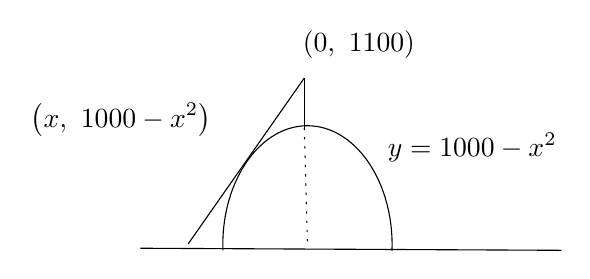
\begin{tikzpicture}[x=0.75pt,y=0.75pt,yscale=-1,xscale=1]
%uncomment if require: \path (0,300); %set diagram left start at 0, and has height of 300

%Straight Lines [id:da5723816642656105] 
\draw    (161,231) -- (364,232) ;
%Shape: Arc [id:dp6981731539336795] 
\draw  [draw opacity=0] (200.8,232.01) .. controls (200.77,231.15) and (200.76,230.28) .. (200.75,229.4) .. controls (200.73,197.7) and (218.96,171.99) .. (241.48,171.97) .. controls (264,171.95) and (282.28,197.63) .. (282.31,229.33) .. controls (282.31,230.27) and (282.29,231.19) .. (282.26,232.12) -- (241.53,229.37) -- cycle ; \draw   (200.8,232.01) .. controls (200.77,231.15) and (200.76,230.28) .. (200.75,229.4) .. controls (200.73,197.7) and (218.96,171.99) .. (241.48,171.97) .. controls (264,171.95) and (282.28,197.63) .. (282.31,229.33) .. controls (282.31,230.27) and (282.29,231.19) .. (282.26,232.12) ;  
%Straight Lines [id:da28537975742427224] 
\draw    (240,149) -- (240,173) ;
%Straight Lines [id:da508714474634949] 
\draw    (240,149) -- (184,229) ;
%Straight Lines [id:da9548957625218735] 
\draw  [dash pattern={on 0.84pt off 2.51pt}]  (240,173) -- (241.53,229.37) ;

% Text Node
\draw (279,174) node [anchor=north west][inner sep=0.75pt]   [align=left] {$\displaystyle y=1000-x^{2}$};
% Text Node
\draw (238,125) node [anchor=north west][inner sep=0.75pt]   [align=left] {$\displaystyle ( 0,\ 1100)$};
% Text Node
\draw (107,160) node [anchor=north west][inner sep=0.75pt]   [align=left] {$\displaystyle \left( x,\ 1000-x^{2}\right)$};
\end{tikzpicture}
\\
\\
The slope at point $x$ on the graph is $\frac{dy}{dx} = -2x$. At the same time the slope of the line that goes through the points $(x, 1000-x^2$ and $(0, 1000)$ is $\frac{1100-(1000-x^2)}{0-x}$. So we have to solve an equation for $x$.

\[
\frac{1100-(1000-x^2)}{0-x} = -2x
\]
\[
100+x^2 = 2x^2
\]
\[
x^2 = 100
\]

 The ant begins to see the tower at height $y = 1000-100 = 900$.

\subsection{Problem 4}
\begin{itemize}
 \item[(a)] $y = \frac{x^2}{4p}$, the slope at point $x$ is equal to $\frac{dy}{dx} = \frac{x}{2p}$.
 The tangent line has form $y = \frac{dy}{dx}x + b$. The $y$-intercept is equal to $b$ when $x = 0$. So at point $(x_0, y_0)$ we have an equation:
 \[ y_0 = \frac{x_0}{2p}x_0 + b \]
 \[ b = y0 - \frac{x_0^2}{2p} \]
 \[ \frac{x_0^2}{2p} = 2y_0 \]
 \[ b = y_0 - 2y_0 = -y_0 \]

\item[(b)] Let $A = (0,p)$, $B = (x_0, y_0)$ and $C = (0, -y_0)$.\\
\\
The distance formula $D = \sqrt{(x_2 - x_1)^2 + (y_2 - y_1)^2}$. 
\\ \\
$D_{AB} = \sqrt{x_0^2 + (y_0-p)^2} = \sqrt{x_0^2 + y_0^2 - 2y_0p + p^2} = \sqrt{x_0^2+\frac{x_0^4}{16p^2}-\frac{2x_0^2p}{4p}+p^2} =$ \\ \\ $\sqrt{\frac{16x_0^2p^2+x^4-8x_0^2p^2+16p^4}{16p^2}} = \sqrt{\frac{x_0^4+8x_0^2p^2+16p^4}{16p^2}} = \sqrt{\frac{(x_0^2+4p^2)^2} {16p^2}}=\frac{x_0^2+4p^2}{4p} = $ \\ \\ $\frac{x_0^2}{4p}+p$ \\ \\ \\ \\
$D_{AC} = \sqrt{(-y_0-p)^2} = \sqrt{y_0^2 + 2y_0p + p^2} = \sqrt{\frac{x_0^4}{16p^2} + \frac{2x_0^2p}{4p} + p^2} = $
\\ \\
$\sqrt{\frac{x_0^4+8x_0^2p^2+16p^4}{16p^2}} = \sqrt{\frac{(x_0^2+4p^2)^2}{16p^2}} = \frac{x_0^2+4p^2}{4p} = \frac{x_0^2}{4p} + p$ \\ \\

The triangle is isosceles as $D_{AB} = D_{AC}$.
\newpage
\item[c)]
Let's take reflection point $B$. Without loss of generality we show that ray $BE$ is parallel to the axis. As shown in $(b)$ the triangle $ABC$ is isosceles. The base of triangle is $BC$ and angles $\alpha$ and $\beta$ are equal. Since angles $\alpha$ and $\theta$ are equal by definition, it implies that $\beta = \theta$. Ray $BA$ is parallel to the axis as shown in the picture. That implies that ray $BE$ is also parallel to the axis. 
\begin{figure}
    \centering
    \includesvg{diagram-1.svg}
    \label{fig:enter-label}
\end{figure}
\end{itemize}

\subsection{Problem 5}
\begin{itemize}
\item[a)] 
$V = \frac{(10-t)^2}{5}$ \\ \\ 
$\frac{\Delta V}{\Delta t} = \frac{V(0) - V(5)}{0 - 5} = \frac{20 - 5}{-5} = -3\; l/m$.

\item[b)]
$\frac{dV}{dt} = -\frac{2}{5}(10-t)$ \\ \\
When $t = 5$, then $\frac{dV}{dt} = -2\; l/m$

\subsection{Problem 6}

\begin{itemize}
\item[(19d)] 
\[\lim_{x\to \infty}x\sin\ \frac{1}{x}\]
\[x = \frac{1}{u}\]
\[\lim_{u\to 0}\frac{\sin u}{u} = 1\]

\item[(19f)]
\[\lim_{x \to 0}\frac{\sin^2 x}{3x^2} = \lim_{x \to 0}\left[ \frac{1}{3}\frac{\sin x}{x}\frac{\sin x}{x} \right] = \frac{1}{3}\]
\end{itemize}

\subsection{Problem 7}
\begin{itemize}
\item[a)] 
$D(uvw) = (uv)'w + uvw' = (u'v + uv')w + uvw' = u'vw + uv'w + uvw'$
\item[b)]
$D(u_1u_2 \dots\ u_n) = u_1'u_2 \dots un + u_1u_2' \dots u_n + u_1u_2 \dots u_n'$ \\ \\
Let's prove that statement by induction. The base case is presented in $(a)$. Suppose that the guessed formula for $D(u_1u_2 \dots\ u_n)$ is true. We need to show that it's also true for $D(u_1u_2 \dots\ u_nu_{n+1})$. \\
Let $w = u_1u_2 \dots\ u_n$. \\
Now $D(wu_{n+1}) = w'u_{n+1} + wu_{n+1}' = (u_1'u_2 \dots un + u_1u_2' \dots u_n + u_1u_2 \dots u_n')u_{n+1} + (u_1u_2 \dots\ u_n)u_{n+1}' = u_1'u_2 \dots unu_{n+1} + u_1u_2' \dots u_nu_{n+1} + u_1u_2 \dots u_n'u_{n+1} + u_1u_2 \dots\ u_nu_{n+1}'$.
\end{itemize}

\end{itemize}

\end{document}
